\chapter{西南林业大学研究生学位论文撰写规范}
\label{cha:spec}

为规范我校研究生学位论文(包含研究报告等)编写格式,结合我校实际,制定本研究生学位论文撰写
规范。除特别说明,本规范中所提到学位论文(包含研究报告等)均简称为论文。

\section{基本结构}
\label{sec:basic}

\subsection{封面}%\footnote{见附 1,}
\label{sec:cover}

按研究生院规定统一制做(见图~\ref{fig:cover-phd})。

\begin{enumerate}
\item 论文题目:应能概括整个论文最重要的内容,要求具体、扼要、简明,严格控制在 25 字以内。
\item 学科专业:以国务院学位委员会批准的学科专业目录中的学科为准,一般为二级学科,按一级学
  科培养的则填一级学科。
\item 学号和作者姓名。
\item 指导教师: 未经学位评定委员会遴选且在研究生院备案的合作指导教师,不得在学位论文上署名;
  署名的合作指导教师人数不超过 2 人。
\end{enumerate}

\subsection{扉页}%\footnote{}
\label{sec:title}

按研究生院规定统一制做,包括中文扉页(见图~\ref{fig:titlepage-phd})和英文扉页(见
图~\ref{fig:titlepage-en}),中英文扉页分别单设一页。

\subsection{独创性声明和论文使用授权}
\label{sec:copyright}

单设一页,排在英文扉页后(见图~\ref{fig:copyright})。论文送审前,研究生本人及其导师
均需在独创性声明和论文使用授权上的相应位置签字。

\subsection{中文摘要}
\label{sec:abstract-cn}

硕士论文中文摘要约 800 字左右,博士论文中文摘要约 1500 字左右。内容应包括工作目的、研究方法、
成果和结论,要突出本论文的创造性成果,语言力求精炼。为了便于文献检索,应在本页下方另起一行
注明论文的关键词(3-5 个),格式见图~\ref{fig:Abstract}。

\subsection{英文摘要}
\label{sec:abstract-en}

英文摘要另起一页开始书写,内容与中文摘要相同,格式见图~\ref{fig:Abstract}。

\subsection{目录}
\label{sec:toc}

目录是论文的提纲,也是论文组成部分的小标题,从第一章开始,目录一般列至二级标题,以阿拉伯数
字分级标出。中英文摘要、主要符号表等前置部分不要放在目录里。

\subsection{插图和附表清单}
\label{sec:lof}

论文中如果图、表较多,可以分别列出清单列于目录页之后。图表的清单应有序号、图表名称和页码。

\subsection{主要符号表}
\label{sec:los}

如果论文中使用了大量的物理量符号、标志、缩略词、专门计量单位、自定义名词和术语等,应编写成
注释说明汇集表,中英文要对照。假如上述符号和缩略词使用数量不多,可以不设专门的汇集表,而在
论文中出现时加以说明。

\subsection{绪论或引言}
\label{sec:preface}

在论文主体前,内容为:该研究工作在国民经济中的实用价值与理论意义;本研究主题范围内国内外已
有的文献综述;论文所要解决的问题。通过绪论,读者就能全面了解学位论文的目的、意义和工作内
容。

绪论的主要研究内容的撰写宜使用将来时态,切忌将论文目录直接复制作为研究内容。

\subsection{论文主体}
\label{sec:body}

写作内容可因研究课题的性质而不同,一般包括:理论分析、计算方法、实验装置和测试方法、对实验
结果或调研结果的分析与讨论,本研究方法与已有研究方法的比较等方面。内容应简炼、重点突出,不
要叙述专业方面的常识性内容。各章节之间应密切联系,形成一个整体。

\subsection{结论}
\label{sec:conclusion}

论文的结论是最终的、总体的结论,应包括论文的核心观点。要认真总结自己的创造性工作,阐述本研
究内容的创新性成果在本领域内的地位、作用和意义,并且要交代研究工作的局限,提出未来工作的意
见或建议。应严格区分研究生本人的成果与他人的科研工作。

结论具有相对的独立性,不应是对论文主体中各章小结的简单重复,要与绪论相呼应。结论的措辞要准
确、严谨,不能模棱两可,避免使用“大概”、“或许”、“可能是”等词语;不应有解释性词语,而应直接
给出结果。常识性的结果或重复他人的结果不应作为结论。

\subsection{参考文献}
\label{sec:bib}

只列作者直接阅读过、在论文中被引用过、正式发表的文献资料。参考文献按文中引用标注的顺序放在
致谢后,不得放在各章之后。

\subsection{附录}
\label{sec:app}

可以包括正文内不便列出的冗长公式推导;以备他人阅读方便所需的辅助性数学工具或表格;重复性数
据图表;计算程序及说明等。

\subsection{作者简历}
\label{sec:author}

内容一般包括:姓名、性别、出生日期、籍贯、最后学历(学位)、毕业院校、工作经历;在学期间参
加的研究项目、发表论文、申请专利、获奖情况等。

\subsection{导师简介}
\label{sec:boss}

包括姓名,性别,出生年月,籍贯,职称,社会职务,学术研究情况,获奖及发表论文情况,研究生工
作情况等。

\subsection{在学期间取得的与学位论文相关的研究成果}
\label{sec:pub}

只列出研究生在攻读学位期间获得的与论文内容相关的学术成果(含发表和已录用的学术论文、获奖、
申请和授权专利、鉴定科研项目)。著作及学术论文等的书写格式要求与参考文献相同。

\subsection{致谢}
\label{sec:ack}

致谢对象限于在学术方面对论文的完成有较重要帮助的团体和个人(不超过300 字)。

上述第\ref{sec:author}、\ref{sec:boss}、\ref{sec:pub}、\ref{sec:ack}等诸节内容要分页单列。

\section{书写规定}
\label{sec:writing}

\subsection{语言表述}
\label{sec:expression}

\begin{enumerate}
\item 论文应层次分明、数据可靠、文字简练、说明透彻、推理严谨、立论正确,避免使用文学性质的带感情色彩的非学术性词语。
\item 论文中如出现非通用性的新名词、新术语、新概念,应作相应解释。
\end{enumerate}

\subsection{标题和层次}
\label{sec:layer}

\begin{enumerate}
\item 层次要清楚,以少为宜,应根据实际需要选择。
\item 博士论文按“章、节”撰写,每章应另起一页。各章节标题要突出重点、简明扼要,不要超过一行,
  标题中不加标点符号。标题中尽量不采用英文缩写词,必须采用时应使用本行业的通用缩写词。见
  表~\ref{tab:layer-phd}。
\item 硕士论文正文一般按“1、1.1” 撰写,每 1 级标题另起一页。各章节标题要突出重点、简明扼要,
  不要超过一行,标题中不加标点符号。标题中尽量不采用英文缩写词,必须采用时应使用本行业的通
  用缩写词。见表~\ref{tab:layer-msc}。
\item 层次代号的格式如表\ref{tab:layer-phd}、\ref{tab:layer-msc}所示。
\end{enumerate}

\begin{table}[H]
  \centering\caption{博士论文层次代号的格式规范\label{tab:layer-phd}}
  \begin{tblr}{width=\linewidth,colspec={clX},hlines,vlines,%
      cell{3}{3}={r=3}{l},row{1}={c} }
    层次名称   & 示例         & 备注 \\
    章         & 第一章 XX…X  & 章名居中书写,章名之间空 1 个半角字符 \\
    一级节标题 & 1.1 XX…X     & 节序顶格书写,与标题名间空 1个半角字符,阐述内容另起一段书写 \\
    二级节标题 & 1.1.1 XX…X   & \\
    三级节标题 & 1.1.1.1 XX…X & \\
  \end{tblr}
\end{table}
    
\begin{table}[H]
  \caption{硕士论文层次代号的格式规范\label{tab:layer-msc}}
  \begin{tblr}{width=\linewidth,colspec={clX},hlines,vlines,%
      cell{2}{3}={r=4}{l},row{1}={c} }
    层次名称   & 示例         & 备注 \\
    1 级标题   & 1   XX…X     & 序顶格书写,与标题名间空 1 个半角字符,阐述内容另起一段书写  \\
    2 级标题   & 1.1 XX…X & \\
    3 级标题   & 1.1.1 XX…X & \\
    4 级标题   & 1.1.1.1 XX…X & \\
  \end{tblr}
\end{table}

各层次的节序及标题不得置于页面的最后一行,只有一行或两行的文字不得做为一页的内容。

\subsection{引用文献标注}
\label{sec:cite}

论文中引用的文献的标注方法遵照 GB/T7714-2005,可采用顺序编码制,也
可采用著者-出版年制,但全文必须统一。

顺序编码制正文中引用文献的标示应置于所引内容最后一个字的右上角,所
引文献编号用阿拉伯数字置于方括号“[ ]”中,用小 4 号字体的上角标,要求如
下:
\begin{enumerate}
\item 引用单篇文献时,如“原核生物的看家基因\textsuperscript{[1]}”。
\item 同一处引用多篇文献时,各篇文献的序号在方括号内全部列出,各序
号间用“,”,如遇连续序号,可标注起止序号。如“……形成了多种数学模型\textsuperscript{[1,5,14-17]}……”
       
\item 当提及的参考文献是句子中的有效成分时,则用小四号字与正文排齐,
如“由文献[8,10-13]可知”。
      
\item 不得将引用文献标示置于各级标题处。
\end{enumerate}
标注著者姓氏和出版年的著者-出版年制,用小四号字与正文排齐,示例如
下:
\begin{enumerate}
\item 16S rDNA 存在于所有原核生物细胞中,被广泛用于细菌的系统学研
究(Schmidt and Reiman, 1994)。
\item Brodaway 等(1986)报道在人工饲料中添加蛋白酶抑制昆虫的生长和发
  育。
\end{enumerate}

\subsection{脚注}
\label{sec:footnote}

采用小五号字,按两端对齐格式书写,单倍行距,段前段后均空 0 行。脚注的序号按页编排,不同页的
脚注序号不需要连续。序号采用“\ring{1},……,\ring{10}”样式,全文格式要统一,详细规定见本页脚注\footnote{脚
  注序号“\ring{1},……,\ring{10}”的字体是“正文”,不是“上标”,序号与脚注内容文字之间空 1个半角字符,脚注的
  段落格式为:单倍行距,段前空 0 行,段后空 0 行,悬挂缩进 1.5字符;中文用宋体,字号为小五
  号,英文和数字用 Times New Roman 字体,字号为 9磅;中英文混排时,所有标点符号(例如逗
  号“,”、括号“()”等)一律使用中文输入状态下的标点符号,但小数点采用英文状态下的样
  式“.”。}。

\subsection{图、表和公式}
\label{sec:floats}

文中的图、表、公式一律采用阿拉伯数字分章连续编号。如:图 2-5,表 3-2,
公式(5-1)等。图表中物理量、符号用斜体。若图或表中有附注,采用英文小
写字母顺序编号,附注写在图或表的下方。

\subsubsection{图}
\label{sec:fig}

\begin{enumerate}
\item 每个图均应有图题(由图序和图名组成),图名在图序之后空 1 个半角字符编写。图中若有分图
  时,分图号用(a)、(b)等表示。
\item 图中各部分说明应采用中文或数字符号,引用的外文图除外,图中中文文字用宋体五号字,英文
  和数字用 Times New Roman 字体,字号宜采用 10.5磅字。同一图内文字使用应统一。
\item 各种类型的图要符合相关标准规定或所在行业的常用画法,同一图上能清楚地区分不同曲线。引
  用文献中的图时,除在正文文字中标注参考文献序号以外,还必须在图题的右上角标注参考文献序
  号。
\item 图居中放置,图题居中置于图的下方。当图题超过一行时,图题仍然居中置于图的下方,但图名
  应左对齐编排。当有分图时,各分图题按序置于主图题下方,主图题和分图题整体居中放置,分图题
  不分段,且分图题之间用分号隔开,当分图题的书写内容超过一行时,回行后应与主图名左对齐开始
  书写。图之前,在正文中必须有关于本图的提示,
  如“见图 1-1”、“如图 1-1 所示”等。
\item 图题不能跨页编排;图与图题为一个整体,不得拆开编排于两页。图处的该页空白不够编排该图
  整体时,则可将其后文字部分提前编写,将图移到下页。有分图时,分图过多不能在一页内编排时,
  可转到下页,但总图题只编排在下页。
\item 图应有自明性。图应与图题文字紧密配合,文图相符,内容正确。选图要力求精练,要注意图的
  整体性和美观性。
\item 有数字标注的坐标图,必须注明坐标单位。
\end{enumerate}

\subsubsection{表}
\label{sec:tab}

\begin{enumerate}
\item 每个表格应有表题(由表序和表名组成)。表名在表序之后空 1 个半角字符,表题中不允许出现
  标点符号。
\item 表中文字为中文时用宋体五号;数字和英文时用 Times New Roman 字体 10.5磅。表之前,在正
  文中必须有相关文字提示,如“见表 1-1”、“如表 1-1所示”。一般情况下表不能拆开两页编排。引用
  文献中的表格时,除在正文文字中标注参考文献序号以外,还必须在表题的右上角标注参考文献序
  号。
\item 表题居中置于表的上方,当表题超过一行时,表题仍然居中置于表的上方,但表名左对齐编排。
  全表如用同一单位,则将单位符号移至表头右上角,加圆括号。表中数据应准确无误,书写清楚。数
  字空缺的格内空着。表内文字或数字上、下或左、右相同时,不允许用“〃”、“同上”之类的写法。
\item 表应有自明性。表中参数应标明量和单位的符号,要注意表的美观性和整体性。
\end{enumerate}

\subsubsection{公式}
\label{sec:eq}

   论文中的公式应另起行,并居中书写,公式的序号右端对齐。文中引用公式
时,一般用“见式(1-1)”或“由公式(1-1)”。公式较长时最好在等号“\(=\)”
处转行,如难实现,则可在\(+\)、\(-\)、\(\times\)、\(\div\)运算符号处换行,换行时运算符号仅
书写于换行式之前,不重复书写。

\subsubsection{参考文献}
\label{sec:refs}

参考文献须在文中标注,并按引用顺序附于文末,建议根据《中国高校自然
科学学报编排规范》的要求书写参考文献,并按顺序编码,即按文中引用的顺序
编码。作者姓名写到第三位,余者写“,等”或“,et al.”。当参考文献为英文
时,作者名在前,缩写;姓在后,全拼,首字母大写。参考文献标注采用顺序编
码制,文献编号用阿拉伯数字置于方括号“[ ]”中,且编号与作者之间空 1 个半
角字符书写。

\paragraph{文献类型标志}

\begin{enumerate}
\item 参考文献类型:期刊文章[J],会议论文[C],专著[M],学位论文[D],报纸文章[N],报告[R],
  专利[P],标准[S];
\item 电子文献类型:数据库[DB],计算机程序[CP],电子公告[EB];
\item 电子文献的载体类型:互联网[OL],光盘[CD],磁带[MT],磁盘[DK]。
\end{enumerate}

\paragraph{几种主要参考文献的格式}

\begin{itemize}
\item 期刊文章:[序号] 作者.文题[J]. 刊名,年,卷号(期号):起-止页码
\item 会议论文:[序号] 作者.文题[C]. 会议论文集名会议地点,会议时间,起-止页码
\item 专(译)著:[序号] 作者.书名[M]. (译者) .出版地:出版者,出版年,起-止页码
\item 学位论文:[序号] 作者.文题[D]. 授予单位所在地:授予单位,授予年,起-止页码
\item 报纸文章:[序号] 作者.文题[N]. 报纸名,出版日期
\item 报 告:[序号] 作者.文题[R]. 报告地:报告主办单位,报告时间.
\item 专 利:[序号] 申请者.专利名[P]. 专利国名,专利种类,专利号,申请或授权日期
\item 技术标准:[序号] 发布单位.技术标准代号.技术标准名称[S]. 出版地:出版者,出版日期
\item 电子文献:[序号] 作者.文题[文献类型标志/文献载体标志]. 出版地或获得地址:出版者,发表
  更新日期或引用日期
\end{itemize}
\medskip%
举例如下:
\begin{itemize}
\item[] [1] 梅树立,陈奎孚,张森文,等. 两点边值问题的 Shannon 小波数值解法[J]. 中国农业大学
  学报, 2002, 7 (2): 12\char`~{}16
\item[] [2] 朱文学. 粮食干燥原理及品质分析[M]. 北京:高等教育出版社,2001,57\char`~{}108
\item[] [3] Dupont B. Bone marrow transplantation in severe combined immunodeficiency with
  an unrelated MLC compatible donor. In: White H J., Smith R, eds. Proceedings of the
  Third Annual Meeting of the International Society for Experimental Hematology.
  Houston: International Society for Experimental Hematology[M], 1974. 44\char`~{}46
\item[] [4] 倪静. 朱砂叶螨线粒体 TcATP6 和 TcATP16 基因的克隆与表达分析[D]. 昆明: 西南林业大
  学,2014, 1\char`~{}45
\item[] [5] 姜锡洲. 一种温热外敷药制备方法 [P]. 中国,发明专利,881056073,1980-07-26
\item[] [6] 中华人民共和国国家技术监督局. GB3100\char`~{}3102. 中华人民共和国国家标准—量与单位[S]. 北
  京:中国标准出版社,1994-11-01
\item[] [7] M. Clerc. Discrete particle swarm optimization: a fuzzy combinatorial
  box[OL]. \url{http://clere.maurice.free.fr/pso/Fuzzy_Discrere_PSO/Fuzzy_DPSO.htm},
  July 16, 2010
\end{itemize}

\subsection{量和单位}
\label{sec:unit}

要严格执行 GB3100-3102-93 有关量和单位的规定(具体要求请参阅《常用量和单位》. 计量出版社,
1996)。论文中某一量的名称和符号应统一,量的符号、常量和变量符号必须采用斜体;计量单位名称
的书写,可以采用国际通用符号,也可以用中文名称,但全文应统一,不要两种混用。计量单位符号,
除用人名命名的单位第一个字母大写之外,一律用小写字母。

不定数字之后可用中文计量单位符号,如“几千克”。表达时刻时应采用中
文计量单位,如“上午 9 点 1 刻”。计量单位符号一律采用正体书写。

\subsection{数字}
\label{sec:dig}

按《关于出版物上数字用法的试行规定》(1987 年 1 月 1 日国家语言文字工
作委员会等 7 个单位公布),除习惯用中文数字表示的以外,一般数字均用阿拉
伯数字,采用 Times New Roman 字体。

\subsection{定理环境和证明环境等}
\label{sec:theorem}

“定理”、“引理”和“证明”等字的字体为黑体,字号为小四,段前空 4 个半角
字符;定理或引理证明完毕后用证毕符号黑色方块“■”表示,证毕符号置于证明
内容最后一行的末尾。

\subsection{攻博/攻硕期间的研究成果}
\label{sec:paper}

\begin{enumerate}
\item 与学位论文相关的主要学术论文、专利和专著等,书写格式与参考文献的书写格式相同;
\item 与学位论文相关的主要科研成果获奖,书写格式如下:
  
  获奖人(排名情况). 项目名称. 获奖名称及等级, 获奖时间。如:
  
  XXX(4). 人工介质雷达罩技术研究. 国防科技进步二等奖, 1997 年
\end{enumerate}

\section{印刷要求}
\label{sec:prn}

\subsection{字数}
\label{sec:wc}

全日制硕士研究生学位论文字数一般 3 万字左右,博士研究生学位论文字数
一般 5 到 10 万字,在职硕士专业学位研究生学位论文字数一般不少于 2 万字。

\subsection{封面}%\footnote{见附 1,}
\label{sec:cov}

学位论文封面全校采用统一格式,按研究生院规定统一制做(见图~\ref{fig:cover-phd})。使用云彩纸,
博士学位论文的封面为封面红色,学术型硕士学位论文封面理学为浅灰色,工学为黄色,农学为浅绿色,
管理学、艺术学和经济学粉红色,专业硕士学位论文林业和农业推广领域封面为绿色,工程硕士淡蓝
色。

\begin{enumerate}
\item 题目:宋体三号,题目一行排不下时可排两行,行间距为 1.5 行;
\item 学科专业、指导教师等:宋体三号,行间距为 1.5 行。
\end{enumerate}

\subsection{扉页}
\label{sec:tit}

\subsubsection{中文扉页}%\footnote{见附 2,}

按研究生院规定统一制做(见图~\ref{fig:titlepage-phd})。
\begin{enumerate}
\item 学位论文题目:宋体二号加粗
\item 作者姓名、指导教师、申请学位级别等:三号宋体加粗,行间距为 1.5
行。当指导教师为多名指导教师时,可以在中文扉页中指导教师的位置处填写相
关信息。
\item 密级:如属保密论文,在中文扉页右上角处注明相应的密级,论文密级为内部、秘密、机密、和绝密。字体:宋体四号。
\end{enumerate}

\subsubsection{英文扉页}%\footnote{见附 3}

按研究生院规定统一制做(见图~\ref{fig:titlepage-en})。

\begin{enumerate}
\item 学位论文题目:字体为 Times New Roman,字号为 18 磅加粗,大写。
\item A Doctor Dissertation (Master Thesis or Master Research Report):字体为Times New Roman,字号为 15 磅,行间距为 1.5 行。
\item 学科专业、作者、指导教师、学院等:字体为 Times New Roman,字号为 16 磅, 加粗,行间距为 1.5 行。
\item 英文扉页只能印制一页。
\end{enumerate}

\subsection{页眉和页码}

\subsubsection{页眉}

\begin{enumerate}
\item 对中文摘要、英文摘要、目录等部分,页眉分别用各部分内容的标题。
\item 从第一章开始,奇数页页眉用“本章标题”,偶数页页眉用“西南林业大学博士学位论文/硕士学位
  论文/硕士研究报告”。
\item 页眉文字为中文时,字体采用宋体五号居中书写;为英文和数字时,采用 Times New
  Roman 字体 10.5 磅居中书写,页眉线为单横线。
\end{enumerate}

\subsubsection{页码}

\begin{enumerate}
\item 中文摘要、英文摘要、目录等前置部分用罗马数字连续编排。
\item 中文摘要、英文摘要和目录,每部分采用双面印制,即正面和背面连续编排页码。若某一部分的
  页数为奇数时,该部分的最后一页单面印制,即该页的背面页为空白,不编页码和页眉。
\item 从绪论(第一章)开始按阿拉伯数字连续编排;第一章以奇数页(第“1”页)开始,第一章开始以
  后连续编排,其他章不是一定以奇数页开始;如第一章最后一页为第 17 页,则第二章就以第 18 页
  开始。
\item 页码位于页面底端,居中书写;字体为 Times New Roman,字号为小五。
\end{enumerate}

\subsection{论文字体、字型及字号要求}

论文中所用中文字体(除各级标题外)为宋体小四号,所用数字和英文为
Times New Roman 12 磅字体。各级标题用黑体。博士论文格式如表\ref{tab:fontspec}所示。

\begin{table}[H]
  \centering
  \caption{论文字体、字型、字号要求\label{tab:fontspec}}
  \begin{subtable}{1.0\linewidth}
    \caption{博士论文}
    \begin{tblr}{width=\linewidth,colspec={clX},hlines,vlines,row{1}={c},rows={m}}
层次 & 示例& 格式要求\\
大标题& 第一章 XXX& 黑体小三\\
一级节标题& 4.1 实验装置和试验方法& 黑体四号\\
二级节标题& 4.2.2 实验装置& 黑体四号\\
三级节标题& 1.3.4.1 协商系统& 黑体小四\\
正文& 实验取得预期效果& {中文宋体小四,数字和英文为\\Times New Roman 字体\\12磅}\\
表题、图题和注& 表 2-1 菌株生理生化特征& {中文宋体五号,数字和英文\\Times New Roman字体\\10.5磅}\\
参考文献及页眉& {西南林业大学\\博士学位论文}& {中文宋体五号,数字和英文\\Times New Roman字体\\10.5磅} \\
{附录、个人简介、\\导师简介、获得\\成果目录和致谢}& &{中文宋体小四,数字和英文为\\Times New Roman字体\\12磅}\\
    \end{tblr}
  \end{subtable}\\[2em]
  \begin{subtable}{1.0\linewidth}
    \caption{硕士论文}
    \begin{tblr}{width=\linewidth,colspec={clX},hlines,vlines,row{1}={c},rows={m}}
      层次& 示例& 格式要求\\
      大标题& 1 XXX& 黑体小三\\
      一级节标& 2.1 实验装置和试验方法& 黑体四号\\
      二级节标& 2.2.2 实验装置 & 黑体四号\\
      三级节标& 1.3.4.1 协商系统 & 黑体小四\\
      正文 & 实验取得预期效果& 同博士论文\\
      表题、图题和注& 表 2-1 菌株生理生化特征& 同博士论文\\
      参考文献及页眉& {西南林业大学\\硕士学位论文}& 同博士论文\\
      {附录、个人简介、\\导师简介、获得\\成果目录和致谢} &&同博士论文\\
    \end{tblr}
  \end{subtable}
\end{table}

\subsection{段落及行间距要求}

\begin{enumerate}
\item 从中文摘要到论文最后一页的段落和标题均取固定值为 1.25 行的行间距,所有段落首行空 4 个
  半角字符起书写内容。
\item 按照标题的不同,分别采用不同的段前段后间距:
  \begin{center}
    \begin{tblr}{colspec={lll},hline{1,2,Z}}
      标题级别 &  段前间距&      段后间距\\
      大标题   & 0.5 行  &  0.5行\\
      一级节标题& 0.5 行 &    0行\\
      二级节标题& 0.5 行 &    0行\\
      三级节标题& 0.5 行 &    0行\\
    \end{tblr}
  \end{center}
  (可适当调节上述标题的段后行距,以利于控制正文合适的换页位置)
\item 若两个标题之间没有文字,第二个标题的段前距设置为 0。
\item 目录及参考文献行间距取固定值为 1.25 倍的行间距。注意不要在一篇参考文献中间换页。
\item 图、表、公式与正文之间对行间距要求如下:
  \begin{enumerate}
  \item 图:中文图题的段前为 0 行,段后为 0 行;英文图题的段前为 1 行,段后为 1 行
  \item 表:中文表题的段前为 1 行,段后为 0 行,英文表题的段前为 1 行,段后为 0 行;
  \item 公式:公式的段前段后为 0 行。
  \end{enumerate}
\end{enumerate}

\subsection{附录、参考文献、个人简介、导师简介、获得成果目录和致谢标题}

黑体小三号,段前 0.5 行,段后 0.5 行。

\subsection{用纸及打印规格}

要求双面印刷,除中英文扉页、独创性声明等须单面印制外。

\begin{center}
  \begin{tblr}{colspec={ccccc},hlines,vlines,%
      cell{1}{1,4,5}={r=2}{c}, cell{1}{2}={c=2}{c} }
    {纸张规格\\(mm)}&{页边距 (mm)}&&{页眉距边界\\(mm)}&{页脚距边界\\(mm)}\\
    &左、右& 上、下 &&\\                
    A4(210×297)& 30& 30& 20& 20\\    
  \end{tblr}
\end{center}

最后提交的论文,应是根据评阅人和答辩委员的意见认真修改过的,文中的错别字率不得超过 1‰;必须
图表清晰(最好是非复印件,尤其是彩图),以确保质量。学位论文是研究生阶段成果的直接体现,需
送往国家图书馆、学校图书馆、档案室归档,永久保存,供人查阅。

\begin{figure}[!ht]
  \centering \fbox{
\includegraphics[width=\linewidth]{cover-phd}}
  \caption{博士论文封面\label{fig:cover-phd}}
\end{figure}

\begin{figure}[!ht]
  \centering\fbox{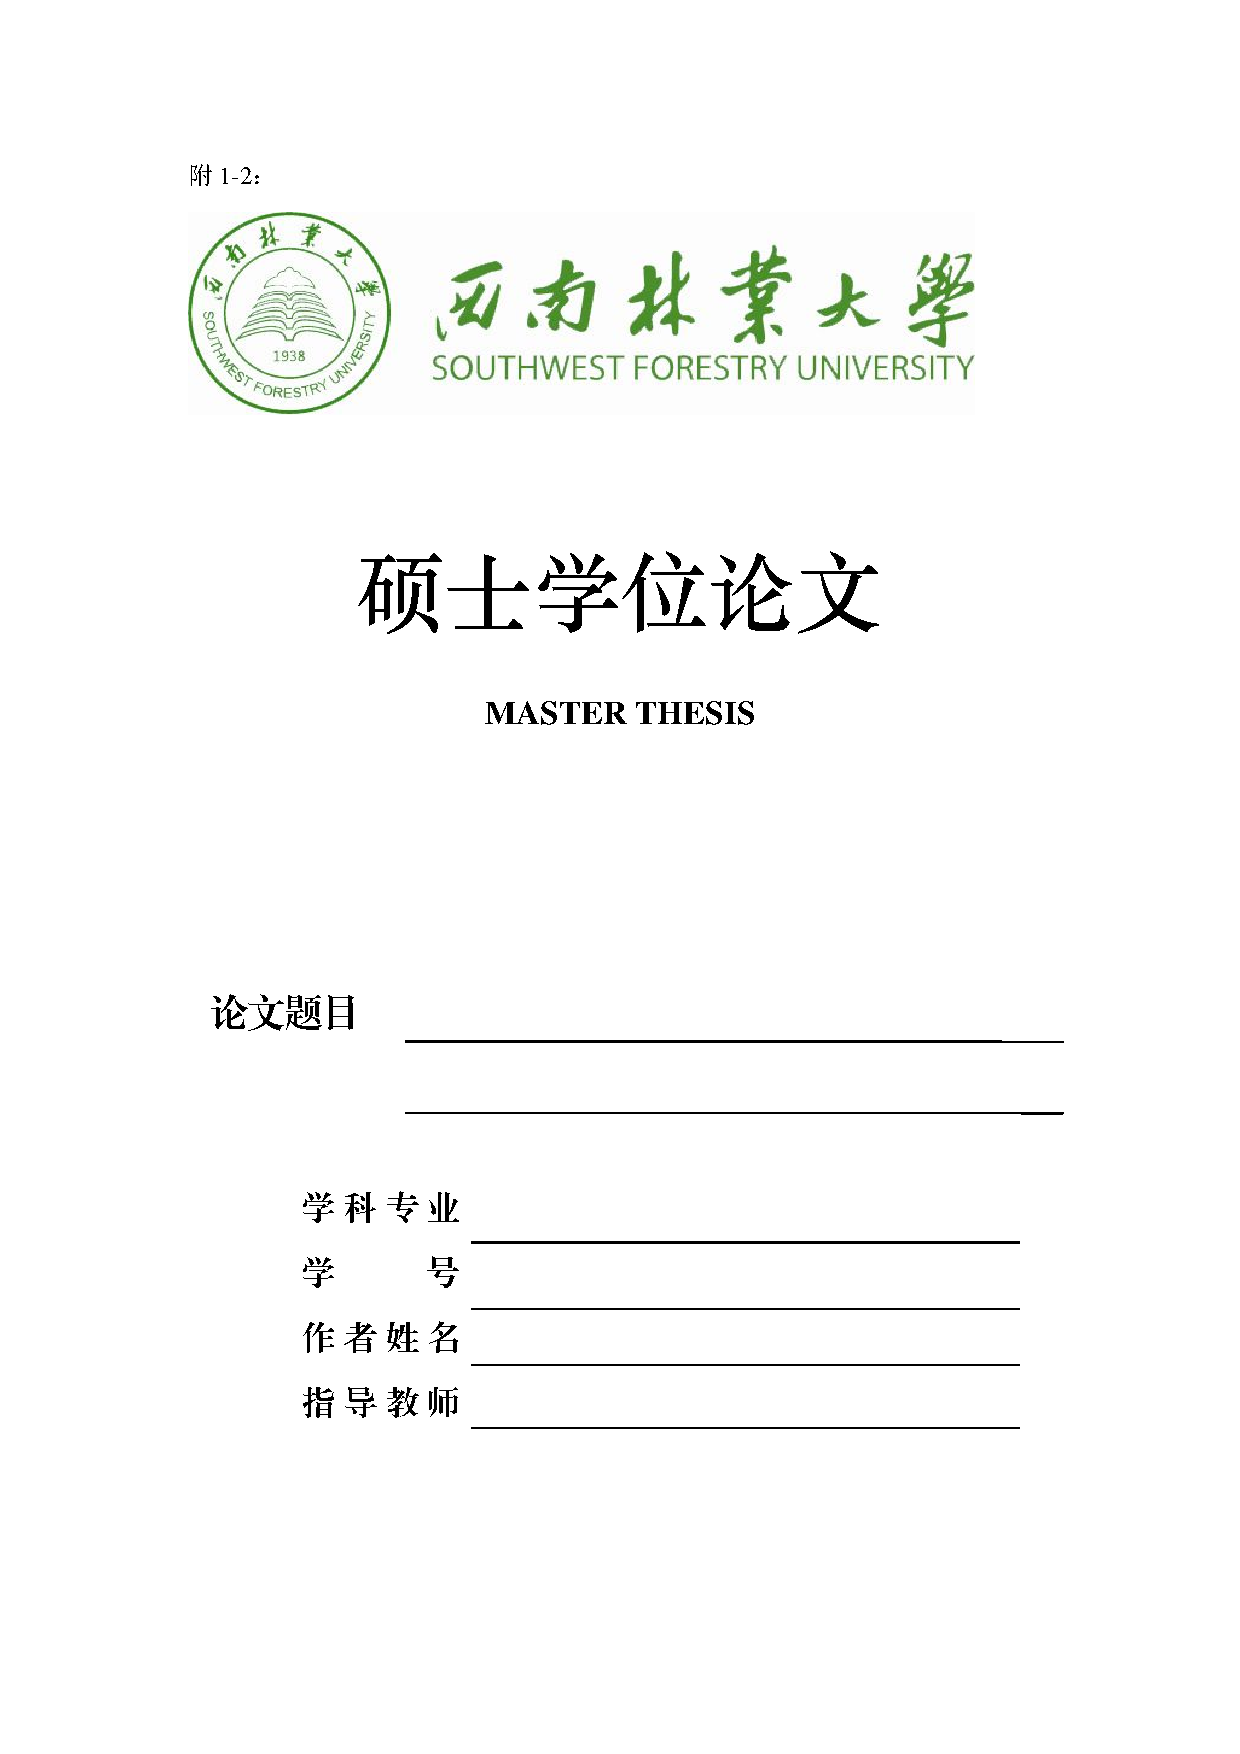
\includegraphics[width=\linewidth]{cover-msc}}
  \caption{硕士论文封面\label{fig:cover-msc}}
\end{figure}

\begin{figure}[!ht]
  \centering\fbox{
\includegraphics[width=\linewidth]{cover-msc2}}
  \caption{专业硕士论文封面\label{fig:cover-msc2}}
\end{figure}

\begin{figure}[!ht]
  \centering\fbox{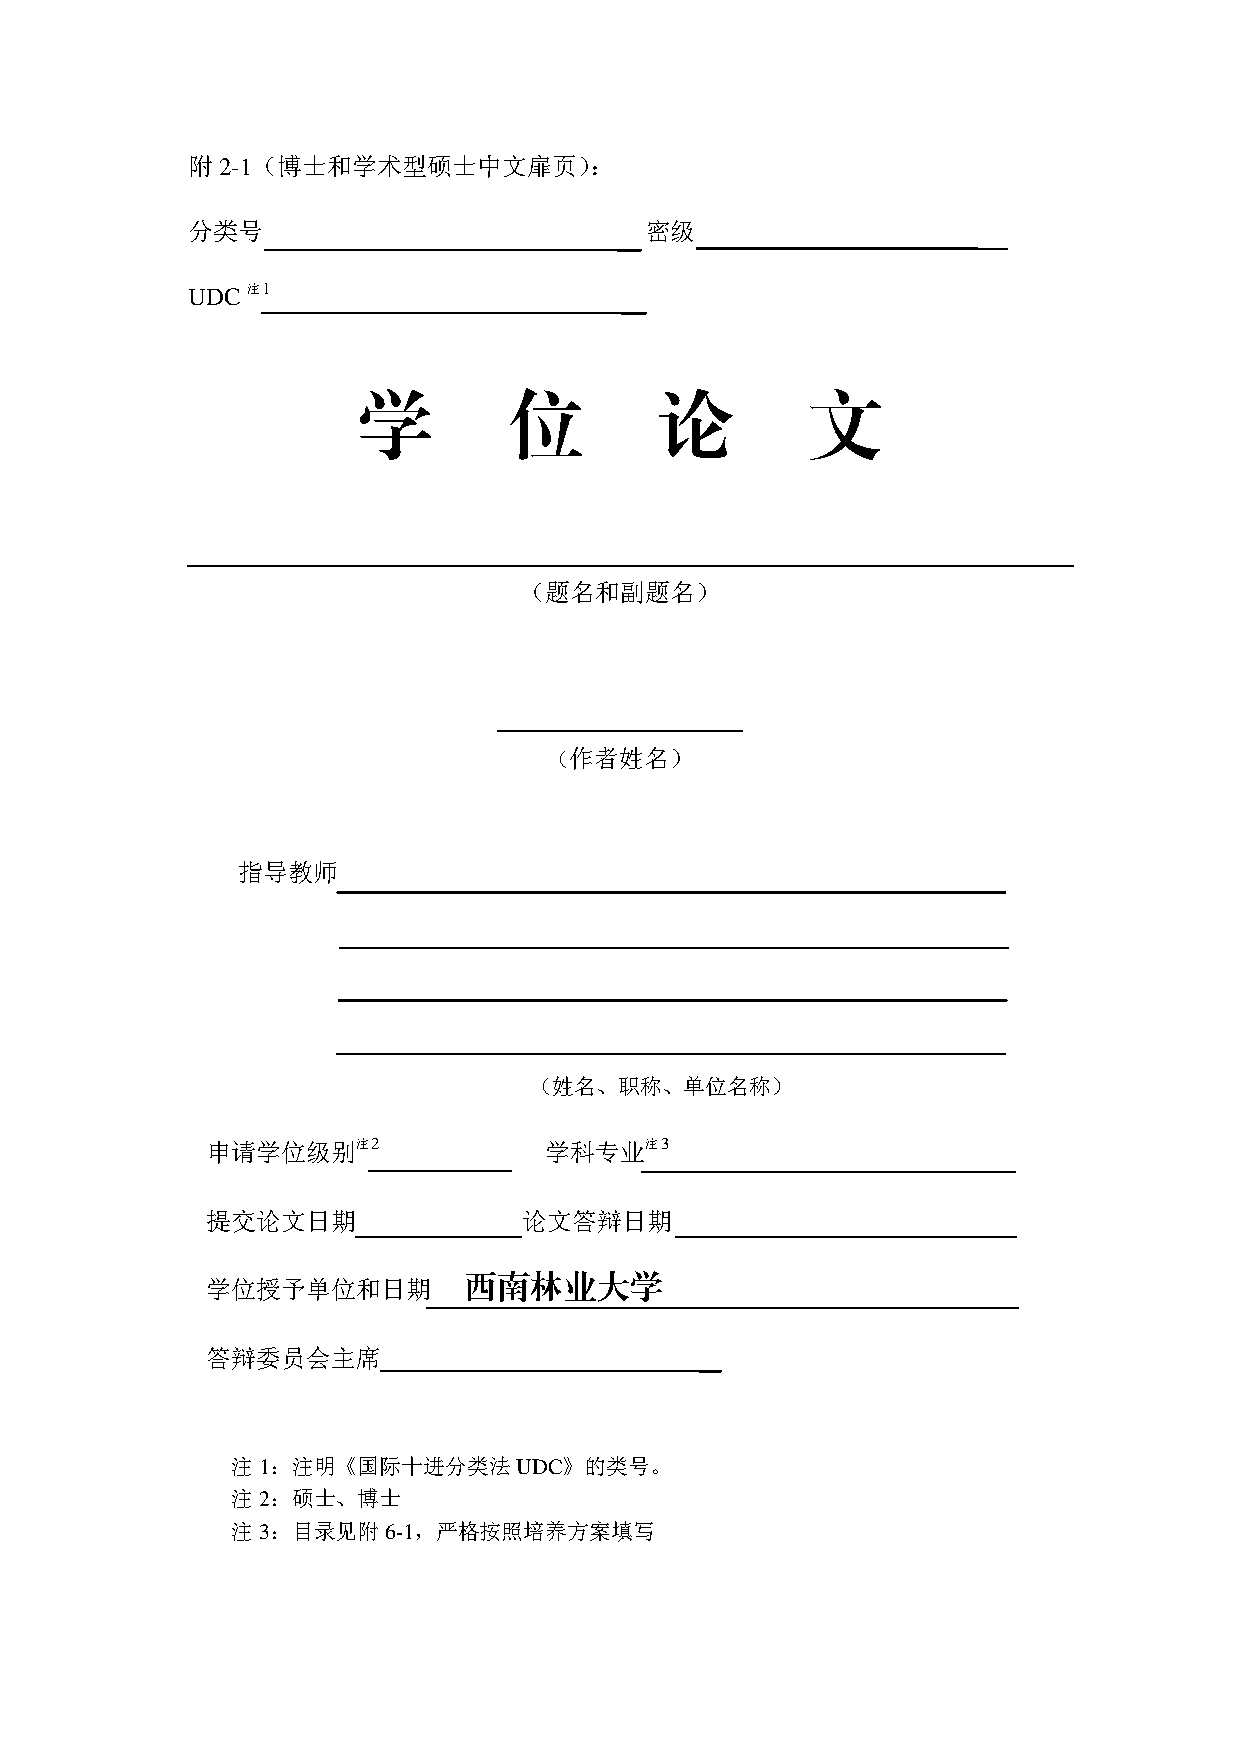
\includegraphics[width=\linewidth]{titlepage-phd}}
  \caption{博士和学术型硕士论文中文扉页\label{fig:titlepage-phd}}
\end{figure}

\begin{figure}[!ht]
  \centering\fbox{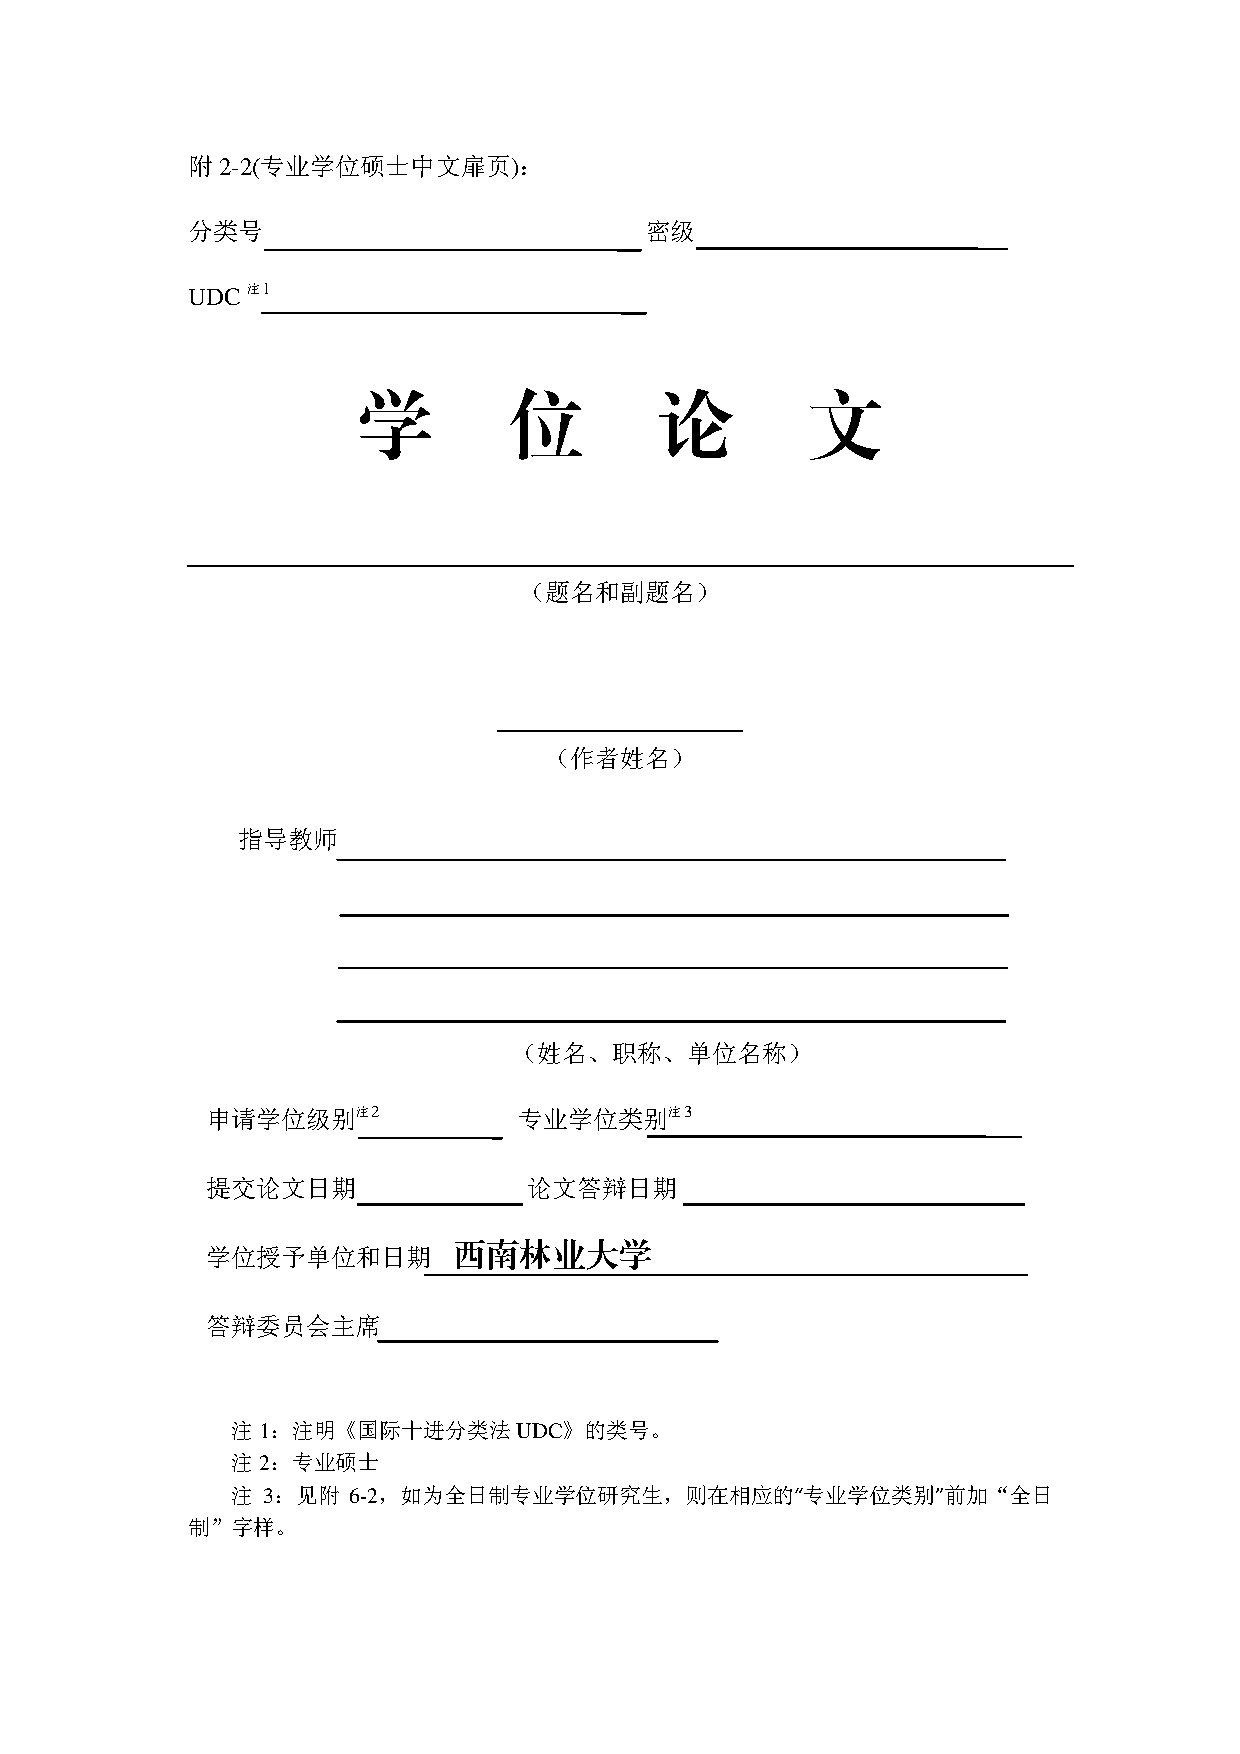
\includegraphics[width=\linewidth]{titlepage-msc2}}
  \caption{专业硕士论文中文扉页\label{fig:titlepage-msc2}}
\end{figure}

\begin{figure}[!ht]
  \centering
  \fbox{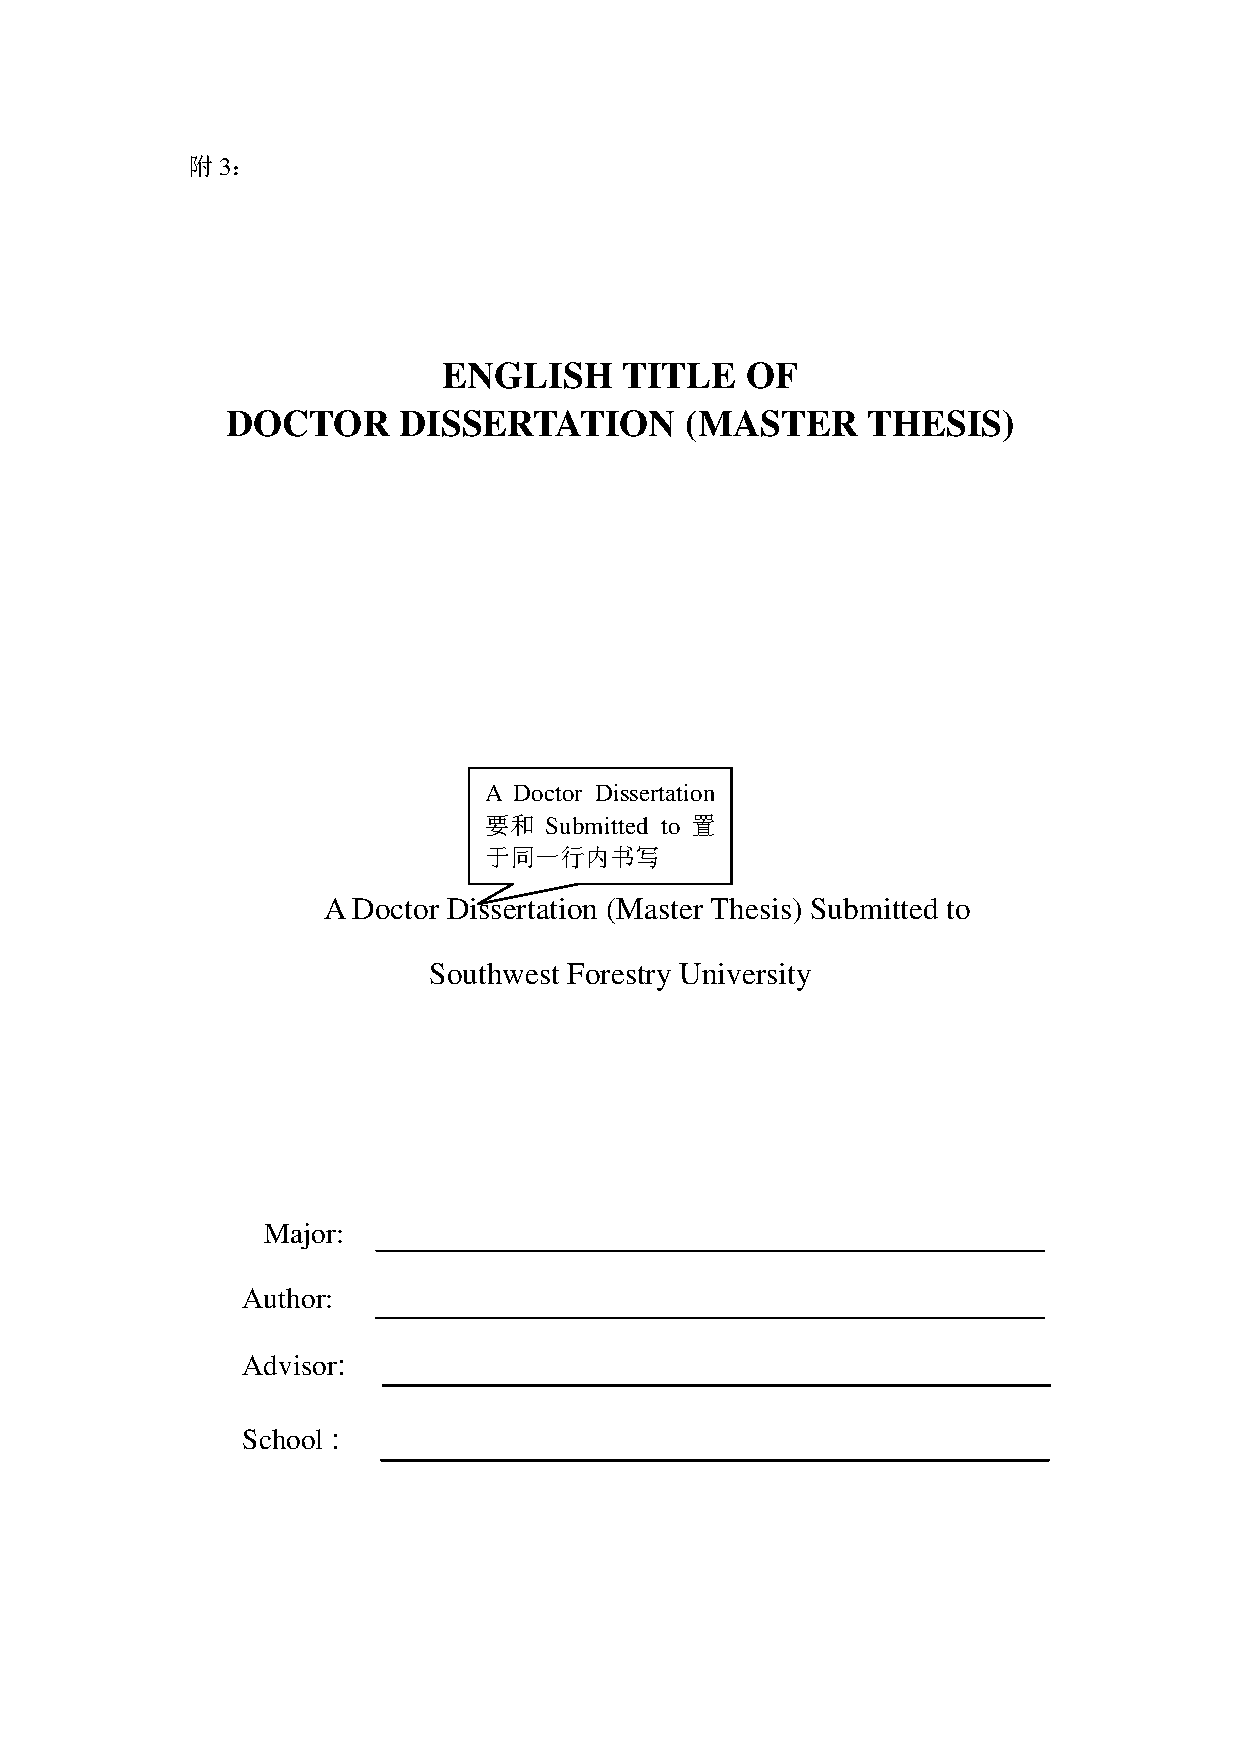
\includegraphics[width=\linewidth]{titlepage-en}}
  \caption{英文扉页\label{fig:titlepage-en}}
\end{figure}

\begin{figure}[!ht]
  \centering
  \fbox{
\includegraphics[width=\linewidth]{copyright}}
  \caption{独创性声明页\label{fig:copyright}}
\end{figure}

\begin{figure}[!ht]
  \centering
  \fbox{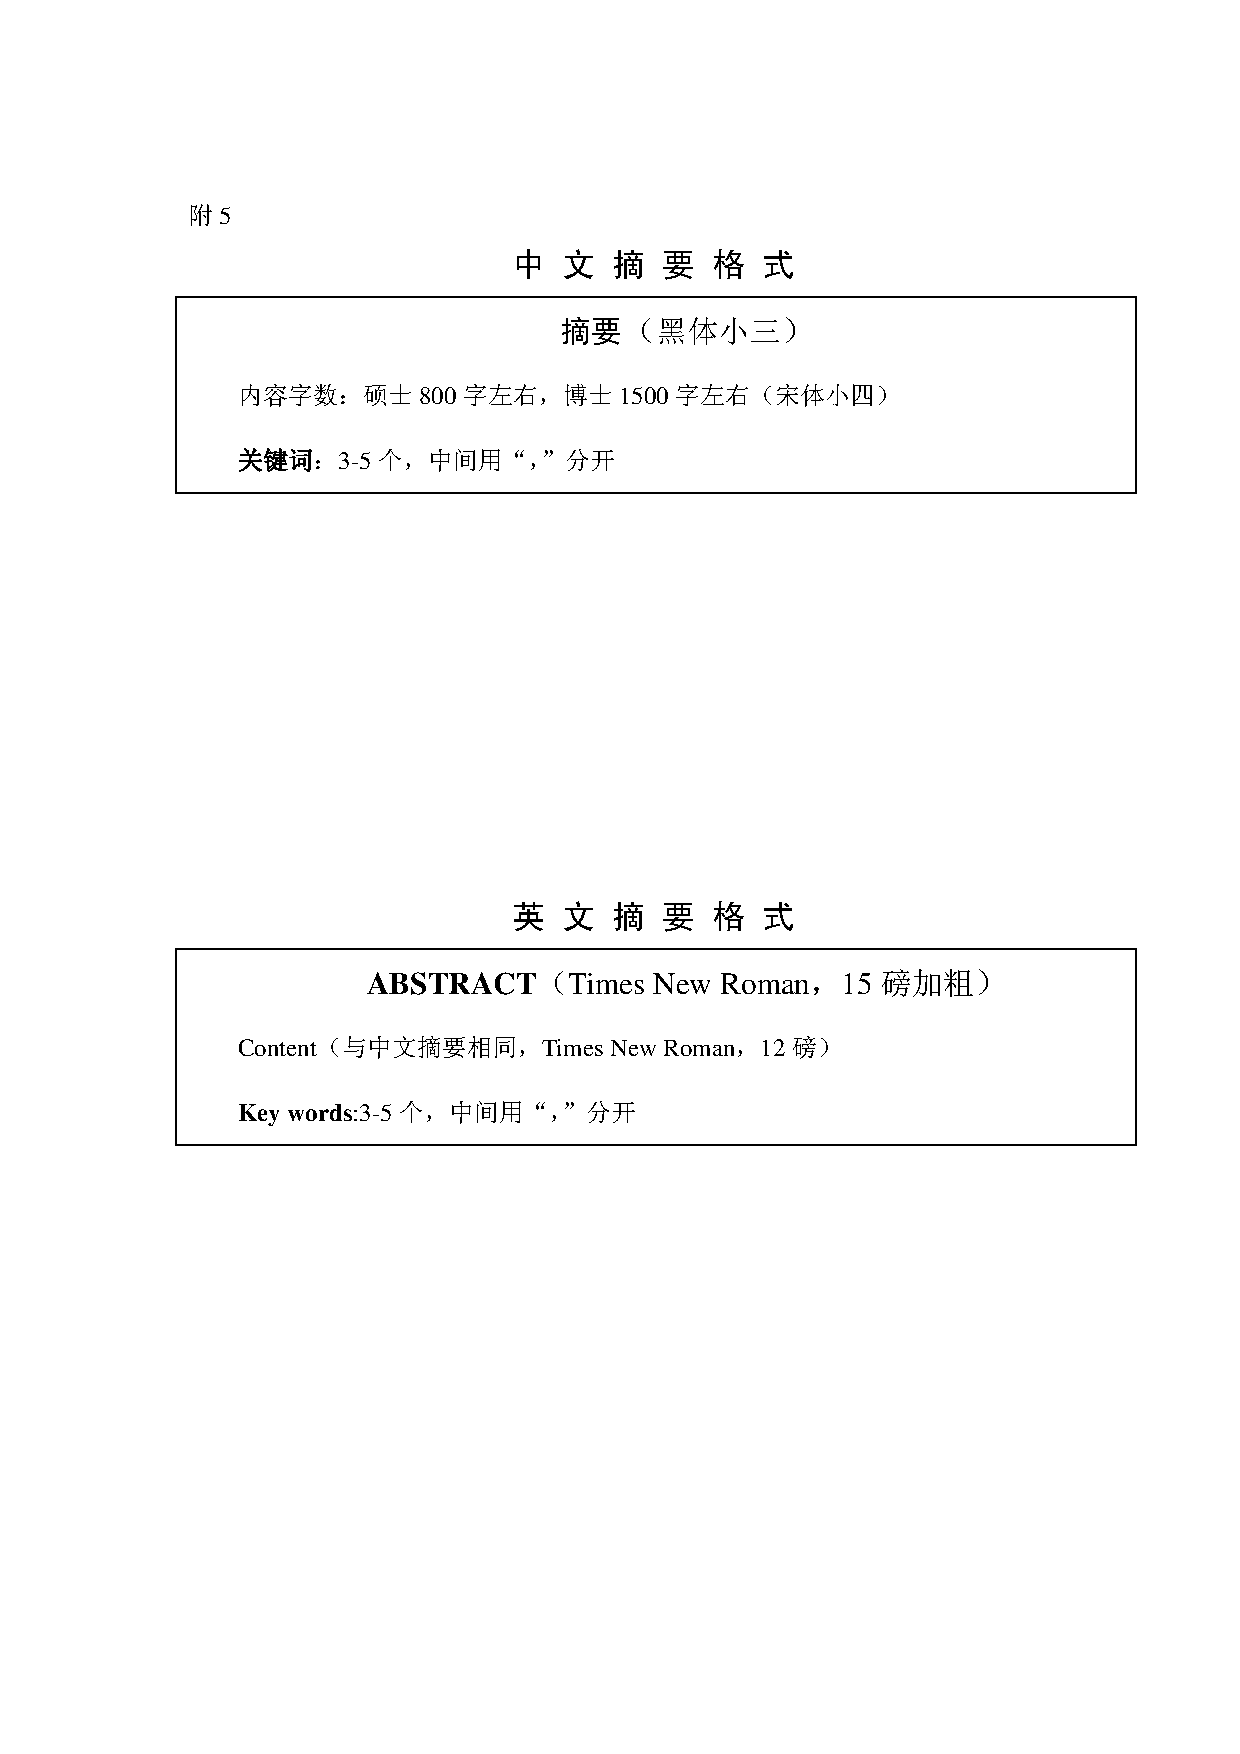
\includegraphics[width=\linewidth]{Abstract}}
  \caption{摘要格式\label{fig:Abstract}}
\end{figure}

%%% Local Variables:
%%% mode: latex
%%% TeX-master: "../example"
%%% End:
